\documentclass[tikz, border=2pt]{standalone}
\usepackage{tikz}
\usepackage{pgfplots}
\begin{document}
    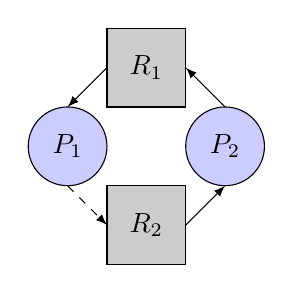
\begin{tikzpicture}
        \draw[fill=blue!20] (-1,0) circle (0.5) node {$P_1$};
        \draw[fill=blue!20] (1,0) circle (0.5) node {$P_2$};
        \draw[fill=black!20] (-0.5,0.5) rectangle ++(1,1) node [midway] {$R_1$};
        \draw[fill=black!20] (-0.5,-1.5) rectangle ++(1,1) node [midway] {$R_2$};
        \draw[-latex] (-0.5,1) -- (-1,0.5);
        \draw[-latex] (1,0.5) -- (0.5,1);
        \draw[-latex, dashed] (-1,-0.5) -- (-0.5,-1);
        \draw[-latex] (0.5,-1) -- (1,-0.5);
    \end{tikzpicture}
\end{document}